\section{Computer Experiments} \label{ch:computer_experiments}
This section describes the setup and configuration of the computational experiments conducted in this study, and the accompanied results. Two types of statistical models, \acrshort{convlstm} and \acrshort{ar}-model are trained and evaluated on an unseen portion of the dataset. 

\subsection{Framework, Structure and Implementation} \label{sec:structure_and_implementations} \label{sec:framework}
%\section{Structure and Implementations} 
The numerical methods used in this study are described in Chapter \ref{ch:num_methods}. The code is available on GitHub in the project repository named ``MS'' on \href{https://github.com/hannasv/MS}{https://github.com/hannasv/MS}. Instructions for downloading reanalysis (ERA5) data using python is provided.

%The repository contains everything need to reproduce the results in this study.
%The experiments are conducted in notebooks and the developed modules are stored in the package ``sciclouds''. Descriptions on how to acquire the data (scripts if possible) and project environment is provided to simplify the process.

The code is developed in Python3.7, a popular language for scientific software development. The source code is stored in the package \textit{sciclouds}, made available on Github trought the project repository. Developed modules draw inspiration from the structure of \textit{scikit-learn} (\cite{sklearn_api}).% and the \textit{keras-tuner} (\cite{chollet2015kerastuner}). 
%The \acrshort{convlstm} is implemented %in \textit{keras} (\cite{chollet2015keras})
%using \textit{tensorflow v 2.0} . %The \textit{keras-tuner} is used to automize the hyperparameter search (\cite{chollet2015kerastuner}). 
The \acrshort{convlstm} is implemented using Tensorflow's keras API (\cite{tensorflow2015}) which simplifies many aspects of building and executing machine learning models. Its implementation and distribution system aware, making the code more versatile. %Easily portable between systems.
The \acrshort{ar}-models are trained and evaluated using self implemented modules. The idea was to utilize the analytical solution of the least squares problem. Many regression modules provide a numerical solution, not the analytical. The python package ``sciclouds'' provides a self implemented version of \acrshort{ar}-models, using the analytical solution to the least squares problem derived in Section \ref{sec:ARmodels}.

Visualizations are generated using \textit{Matplotlib} (\cite{matplotlib}), \textit{Seaborn} (\cite{seaborn}) and maps using the package \textit{Cartopy} (\cite{Cartopy}). Other illustrations are developed using TIkZ, a language used for producing technical illustrations within the environment of LaTEX.

The package versions are documented in the \textit{requirements.txt} and the project environment called ``sciclouds'' is ready for installation. This is a conda environment, the yaml-file lists the Python packages and requirements necessary for running this code. Below you find the code example for cloning the project and installing the environment.

% Included in the readme file on github. 
\begin{verbatim}
git clone https://github.com/hannasv/MS.git
cd MS
conda env create -f environment.yml
conda activate sciclouds
python setup.py install # installing package from source
\end{verbatim}

Supplementary material for remapping satellite data and filtering masks is available in the supplementary repository \href{https://github.com/hannasv/MS-suppl}{https://github.com/hannasv/MS-suppl}. %To make use of all the functionality available trought ``MS'', the supplementary repository needs to be cloned in the same directory.
The filters are generated from within the environment of PyAEROCOM (\cite{pyaerocom}). 


%Complex computations will cause memory growth, dependant on how many intermediate computations it needs to store. This is the case for \acrshort{convlstm}. To speed up the development process the software is developed on a subset of \acrshort{ecc}. Small adjustments needs to be made, running experiments on the entire data. For instance threads deadlock when extracting large amounts of data. This is a precautionary measure to avoid overloading the system. \textbf{Possible to develop code to do Hyperparameter tuning based on }
%For a more detailed description please see the project repository described in Section \ref{sec:structure_and_implementations}.

\subsection{Hardware} \label{sec:hardware}
%How to deal with big datasets that will easily eat up you memory? ``Big data'' involve processing large amounts of data that does not fit into memory. Processing substantial amounts of data require expert knowledge about distributed systems and analysing for system bottlenecks.  %Although theoretically fascinating it remains to see if \acrshort{convlstm} provide a clear practical advantage over the autoregressive models.
%Conducting experiments on big datasets require external computational resources.  
The experiments described below, are conducted on a 
%This study had access to a 
DGX-2 system consisting of 16 NVIDIA Tesla V100 GPUs, each of 32Gb local memory and 1.5Tb shared memory. %The resources was available through the \acrfull{ex3} project hosted at Simula. 
This study was awarded access to 1 GPU and 1024G part of the memory. The data is stored on a \acrfull{rdma} accessed over Infiniband. \textit{The best choice of collective implementation depends upon the number and kind of \acrshort{gpu}s, and the network interconnect in the cluster.} The DGX-2 system is designed for a high level concurrency and scheduling workers competing for system resources.
%The hardware sets the limitations for efficiency of pipelines and training procedure. 
%\textit{NVIDIA V100 GPU -- The eX3 infrastructure includes a DGX-2 system consisting of 16 NVIDIA Tesla V100 GPUs, allowing simultaneous communication between all eight GPU pairs at 300 GBps through the 12 integrated NVSwitches. This gives a theoretical system-wide system bi-directional  bandwidth of 2.4 TBps. All GPUs have 32 GB of local memory (total of 512 GB) and share a 1.5 TB main memory. The total system has 81,920 CUDA cores, and 10,240 Tensor cores delivering 2 Petaflops of tensor performance. The peak performance in double precision is 125 Teraflops.}
%Working on such a monstrosity pose additional challenges related to porting existing code and virtual environments, developing and debugging code. To eventually end up with an%a achieved 
%acceptable level of efficiency and reliability. \textbf{må de siteres? (\cite{ex3docs} and \cite{ex3homepage}).} 
\begin{table}[ht]
    \centering
    \begin{tabular}{c|c}
        Device &  Type  \\ \hline
        GPU & Tesla V100-SXM3-32GB \\
        CPU & DualProcessor AMD Epyc7601 (SMT2) w/2TB ram and 4TB NVMe 
    \end{tabular}
    \caption{Hardware specifications for the environment used on \acrshort{ex3}. Operating system is Ubuntu 18.04.4.}
    \label{tab:hardware_ex3}
\end{table}
%TS: Mye av teksten frem til dette punktet egner seg egentlig bedre i et Appendix
\subsection{Model Setup and Evaluation}
The following sections contain the configurations of the models compiled for this study along with descriptions of hyperparameters. A model is compiled based on a choice of hyperparameters, which is a parameter set used before the training starts, as mentioned in Section \ref{sec:artificial neural networks}. In the search for the best model configuration, different combinations of hyperparameters are evaluated. This is done manually since the choice of architecture can easily overload the system memory resources.
 
A starting point for the \acrshort{convlstm} is the set of architectures provided by \citeauthor{SunAirLSTM} (\citeyear{SunAirLSTM}) described in Section \ref{sec:related_work}. The \acrshort{ar}-models follow a different strategy, starting with the simplest models, and gradually increasing the complexity. %This could have been done using spaced sampling, attempting lags of 1, 2, 5, 10. The result becomes the same, however for large model there might be some time to save.

%it follows the principal of starting with the simplest model possible and increasing the complexity from there. 
%Stopping at architectures where increased complexity don't increase the performance? Know stategies are using spaced sampling, attempting lags of 1, 2, 5, 10. The second is naturally to further investigate regons of lags showing the most promise. 
%on a similar problem, air quality forecasting problem was executed. \citepaper{chollet2015kerastuner} provide suitable software for the automatic hyperparameter tuning. 
%\textbf{Man kjører eksperimenter på mange modeller ved å bruke traning og validations dataset. The choice of model is based on this data basis and then it performance is tested on the test dataset.} 
\subsection{Training, validation and test split}
% Gradient methods are at the heart of every machine learning algorithms -- need 
The partitioning into training, validation and test data is different for the models. \acrshort{ar}-models are computed based on an analytical solution, so there is no need for validation data. 

Both models are tested on 2014 to 2018. The \acrshort{ar}-model is trained on the period 2004 to 2013, while the \acrshort{convlstm} is trained on  2004 to 2011 and validated on 2012 to 2013. \textbf{The validation data is necessary because of the numerical approximation used in ConvLSTM when optimising.} The test period was chosen based on the assumption that the latest period is most representative for the climate in the near future. Another minor difference for the datasets prepared for the \acrshort{ar} and the \acrshort{convlstm}-models. The order of the \acrshort{ar}-model determines the length of the training sequence. All samples with gaps in the requested sequence are disregarded causing a reduction in the data basis for a model of a particular order, determined by the number of lags. For the \acrshort{convlstm} these gaps are filled with an out-of-sample value, $c=1.5$. 

The downloaded size of \acrshort{ecc} is 17Gb, stored in \acrshort{netcdf}-files. 
In comparison to related works by \citeauthor{precip_nowcasting} (\citeyear{precip_nowcasting}) and \citeauthor{SunAirLSTM} (\citeyear{SunAirLSTM}), using datasets of size X and Y respectively. A method for training deeper models on datasets is to reduce the spatial or temporal resolution. This is done in precipitation nowcasting, moving from 300x300 pixels to 100x100, based on the argument that this  removes noise. Since cloud cover has an average lifetime as mentioned in Section \ref{sec:cloud_in_climate_system} I argue that \acrshort{ecc} cannot be reduced without significant loss of information. \textbf{Make this a more accurate comparison between the three datasets in volumes.}

\subsubsection{Autoregressive models (AR)}
The set of hyperparameters available for \acrshort{ar}-models are
%A set of models are compiled by varying components such as
standard scaling the predictors, transforming the target, the inclusion of intercept, order of the models and environmental variables. Varying combinations of these parameters results in the set of models used in this part of the experiments. A summary of the performance of the calibrated models is provided in Figure \ref{fig:results_ar_models}. Keep in mind that one \acrshort{ar}-models is the aggregation of 13041 individual regression models. The displayed score is an average over the entire grid, resulting in the average pixels score.

%Time consuming task because of the high number of matrix inversions. A double for loop over this takes to long and \textbf{mention the version of paralelization used on this problem}.

\subsubsection{Feature Scaling} \label{sec:scaling_predictors}
%Feature standardization makes the values of each feature in the data have zero-mean 
Feature scaling is used to standardise the predictor variables.
%By subtraecting the mean and dividing by the variance, t
Applying Equation \eqref{eq:scaling_data} to the predictors reshapes the distribution toward a standard normal distribution with zero mean and unit variance. 
%Data transformation can be beneficially in an attempt 
The transformation offers an additional benefit of increased numerical stability. %When applied the predictors is transformed according to the following Equation \ref{eq:scaling_data}. 
The feature scaling is applied after the partitioning into training and test datasets, and the mean and standard deviation are computed based on the training set. In this manner the trained model avoids sneak peaking at the test data, resulting in a unrepresentative measure on performance.
\begin{equation} \label{eq:scaling_data}
    \mathbf{x} = \frac{\mathbf{x} - \bar{\mathbf{x}}}{\text{STD}(\mathbf{x})}
\end{equation}
where $\bar{\mathbf{x}}$ is the average and STD is the standard deviation. 
The model is trained to find relations in transformed data. Before making predictions based on test data it needs to be transformed, using the mean and standard deviation from the training sample.

\subsubsection{Transforming target} \label{sec:transforming_target}
A trick to avoid predicting unphysical values is fitting against a transformed target. In this study, the target, \acrfull{cfc} ranges from 0 to 1. By applying the inverse sigmoid transformation, see Equation \eqref{eq:inv_sigmoid} the target takes values from the entire real axis $(-\infty, \infty)$. 
\begin{equation} \label{eq:inv_sigmoid}
   \sigma^{-1} \left( x \right) = ln \left(\frac{x}{x - 1 + \epsilon} \right)
\end{equation}
where $\epsilon = 0.01$ \textbf{TODO: update this number} is precaution for when $x=1$ and division by zero would occur. 
The inverse transformation of this is ordinary sigmoid, see Equation \eqref{eq:sigmoid}. By applying this equation values return to the range from 0 to 1. Thereby alleviating predictions of out-of-sample values. The graph is displayed in Figure \ref{fig:activation_function_example}. The sigmoid function is described in Section \ref{sec:artificial neural networks} in the context of its abilities as an activation function in machine learning models. 

\subsubsection{Lags and Environmental variables}
The dataset for a particular model is a combination of the number of lags (order of model) and environmental variables such as $t2m$, $sp$, $q$ and $r$ \textbf{(TODO alle andre plasser har du skrevet det helt ut)} is included. The environmental variables never appear in isolation.
Order the number of time steps of previous cloud cover includes as predictors. All models are trained either on the full set of environmental variables or none of them, such that no partial inclusion of environmental variables occurs. 

\section{Til Trude. Resten er en kladd - jeg har lagt inn notater for å få en følelse på hvordan det blir seende ut til slutt. Noen plot er kun dummy data evt. screenshot fordi resultatene ikke er klare. Du må gjerne komme med inspill på ideene.}

\subsubsection{Experimental setup (AR-models)}
The naming conventions used $AR_{STB_L}$ or $TR_{STB_L}$. B stands for bias, T for scaling predictors, S for sigmoid transformation of the target and L for the number of lags, previous timestep of cloud cover included. AR og Tr describe whether the environmental variables are included in the dataset of not. %This description elaborated in Table \ref{tab:ar_model_config}.
To make it easier to understand the naming convention used, Table \ref{tab:ar_model_config} shows a three examples of the naming conventions udes in this study. %\acrshort{ar}-models included in this study.
Inherited from the nature of the transformation of the predictors the hyperparameters bias and transform is mutually exclusive. The bias is zero when transformation of predictors are applied. 

\begin{table}[h]
    \centering
    \resizebox{\textwidth}{!}{%
    \begin{tabular}{cccccc}
    \cline{2-6}
     & \textbf{Scaling predictors} & \textbf{Transforming target} & \textbf{Lag} & \textbf{Environmental variables} & \textbf{Bias}\\ \hline
    \multicolumn{1}{c}{\textbf{$TR_{SB_1}$}} & \checked & $\times$  & 1 & $\times$ & \checked   \\ \hline
    \multicolumn{1}{c}{\textbf{$AR_{SB_0}$}} & \checked & $\times$  & 0 & \checked  & \checked  \\ \hline
    \multicolumn{1}{c}{\textbf{$AR_{SB_1}$}} & \checked & $\times$  & 1 & \checked & \checked  \\ \hline
    %\multicolumn{1}{c}{\textbf{$AR_{SB_2}$}} & \checked & $\times$  & 2 & \checked & \checked  \\ \hline
    %\multicolumn{1}{c}{\textbf{$AR_{SB_3}$}} & \checked & $\times$  & 3 & \checked & \checked  \\ \hline
    \multicolumn{1}{c}{\textbf{$AR_{SB_4}$}} & \checked & $\times$  & 4 & \checked & \checked  \\ \hline
    \end{tabular}%
    }
    \caption{Configuration of \acrshort{ar}-models. $\times$ denoted not applied, \checked denotes applied. \textbf{Bruk denne for tre eksempler, gjør de mer ulike, velg gjerne best ++ .}}
    \label{tab:ar_model_config}
\end{table}

\begin{figure}
    \centering
    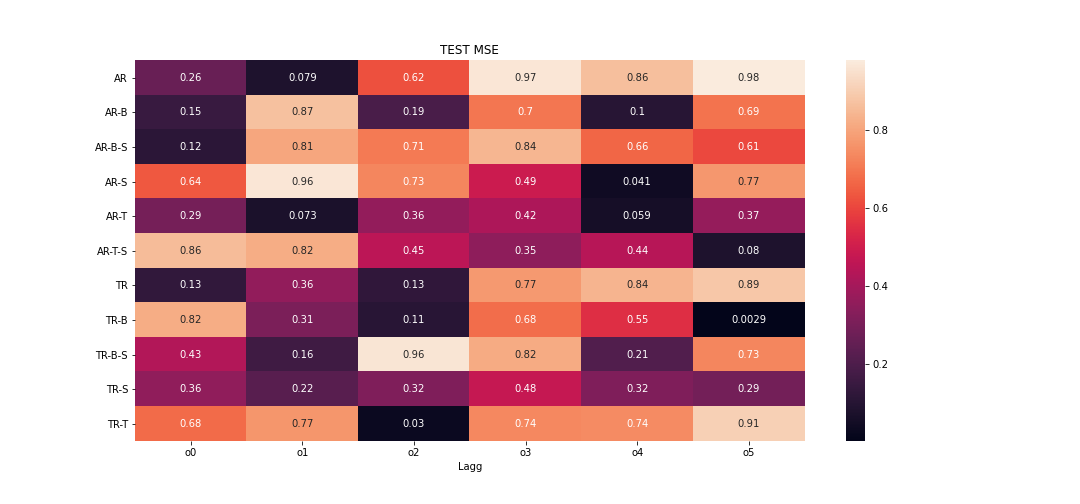
\includegraphics[scale = 0.5]{python_figs/MSE_score_AR_models.png}
    \caption{MSE score for a set of configured AR models}
    \label{fig:results_ar_models}
\end{figure}

Mention that the results are computed by using Equations \eqref{eq:mse} and \eqref{eq:mae}, setting the parameters $m = 81$, $n=161$ and $t=\text{seq length}$. 

\begin{figure}
    \centering
    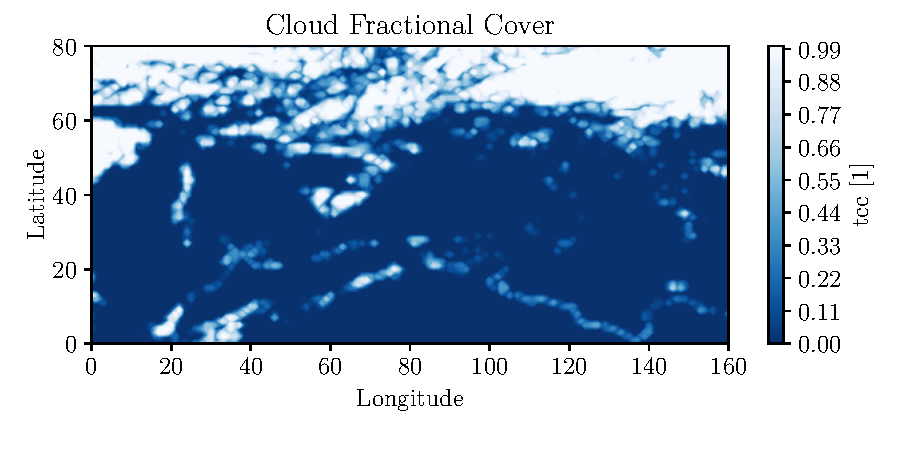
\includegraphics{python_figs/example_artefact.pdf}
    \caption{Reuse this plotting routine to plot the distributed MAE score of the overall best model, \textbf{named X}.}
    \label{fig:grid_mse_best_model}
\end{figure}

\begin{enumerate}
    %\item \textbf{TODO: For the best model plot a grid og MAE and look for patterns n the geographical varying performance.}
    %\item \textbf{Check magnitude of weights and determine/discuss whether any of them can be excluded. Include this as a table}
    \item \textbf{Rename bias to intercept? write bias (intercept)!}
\end{enumerate}

\begin{table}[hp]
    \centering
    \resizebox{\textwidth}{!}{%
    \begin{tabular}{cccccc}
    \cline{2-6}
     & \textbf{W1} & \textbf{W2} & \textbf{W3} & \textbf{W4} & \textbf{W5} \\ \hline
    \textbf{Best model} & 0.3424 & 0.5 & 0.439839   & 0.83247 & 0.98347984 \\ \hline
    \end{tabular}%
    }
    \caption{Add the weights of the best model.}
    \label{tab:weights_best_model}
\end{table}

\subsection{Convolutional LSTM (ConvLSTM)}

The formulation of the air quality forecasting problem presented by  \citeauthor{SunAirLSTM} is similar to the formulation of the cloud fractional cover prediction problem presented in this project. %The machine learning experimental setup is adopted from the paper \citepaper{SunAirLSTM}.
% Endrer på arkitekturen - denne bruker -train - validation - test, en hvis prosentandel a
A lot of architectural decisions such as batch size, sequence length, number of filters and number of layers can cause the \acrshort{gpu} to run out of memory. In these cases the compiled model is not trainable. Between each layer is a Batch Normalization layer. According to the paper \citepaper{ioffe2015batch} this should simplify the training process. Padding same is applied to all layers, to make sure the input and output dimensions are the same. This is described in more detail in Section \ref{sec:padding}. The feature was added between each layer. The dataset is partitioned into subsets called batches. The batch size is the number of samples a weight update is based on. Epochs is the number of times the model loops over the entire dataset. The sequence length is the number of timestamps a model aims to learn to predict. Number of hidden states it the number of filters it learns in each layer. Cite Section \ref{sec:convolutional neural network} for description of hidden states. 
The filter size determines the number of neighbours influencing an activation. Using kernel 1x1 results in the state-to-state transitions, similar to \acrshort{ar}-models without interactions between adjacent pixels. A more detailed description on this is provided in Sections \ref{sec:convolutional neural network} to \ref{sec:convolutional_lstm}. \textbf{Look in the model on other hyperparameters set as constants, like weight init +++ no shuffle on input data, should not help with may epochs then?}

\subsubsection{Experimental setup (ConvLSTM)}
Models are given names based on an extension of the convention from \citepaper{precip_nowcasting}. The paper introduces the convention ConvLSTM-hidden states-filter$\times$filter, adding the batch size and sequence length as tunable parameters. The resulting naming convention is \newline $ConvLSTM-B_{x}-SL_{y}-hidden states-filter$\times$filter$

\begin{table}[hp]
    \centering
    \resizebox{\textwidth}{!}{%
    \begin{tabular}{cccccc}
     & \textbf{Sequence Length} & \textbf{Batch Size} & \textbf{Hidden States} & \textbf{Kernels} & \textbf{Num. Parameters} \\ \hline
    \textbf{$ConvLSTM-B_{5}-SL_{24}-256-3\times3-256-3\times3$} & 24 & 5 & [256, 256]   & [3, 3] & 98347984 \\ \hline
    \textbf{$ConvLSTM-B_{15}-SL_{24}-256-5\times5-256-5\times5$} & 24 & 15 & [256, 256]  & [5, 5] & 4244308 \\ \hline
    \textbf{$ConvLSTM-B_{10}-SL_{24}-128-1\times1-128-1\times1$} & 24 & 10 &  [128, 128] & [1, 1] & 0927502 \\ \hline
    \textbf{$ConvLSTM-B_{5}-SL_{6}-64-3\times3-64-3\times3$} & 6 & 5 & [64, 64]      & [3, 3] & 9472 \\ \hline
    \textbf{$ConvLSTM-B_{5}-SL_{6}-256-3\times3-256-3\times3$} & 6 & 5 & [64, 32]      & [3, 3] & 380495 \\ \hline
    \textbf{$ConvLSTM-B_{5}-SL_{6}-8-3\times3-8-3\times3-8-3\times3$} & 6 & 5 & [8, 8, 8]     & [3, 3, 3] &  20934802\\ \hline
    \end{tabular}%
    }
    \caption{Give three examples to simplify the explanation of configurations and models.}
    \label{tab:convlstm_config}
\end{table}

\begin{figure}
    \centering
    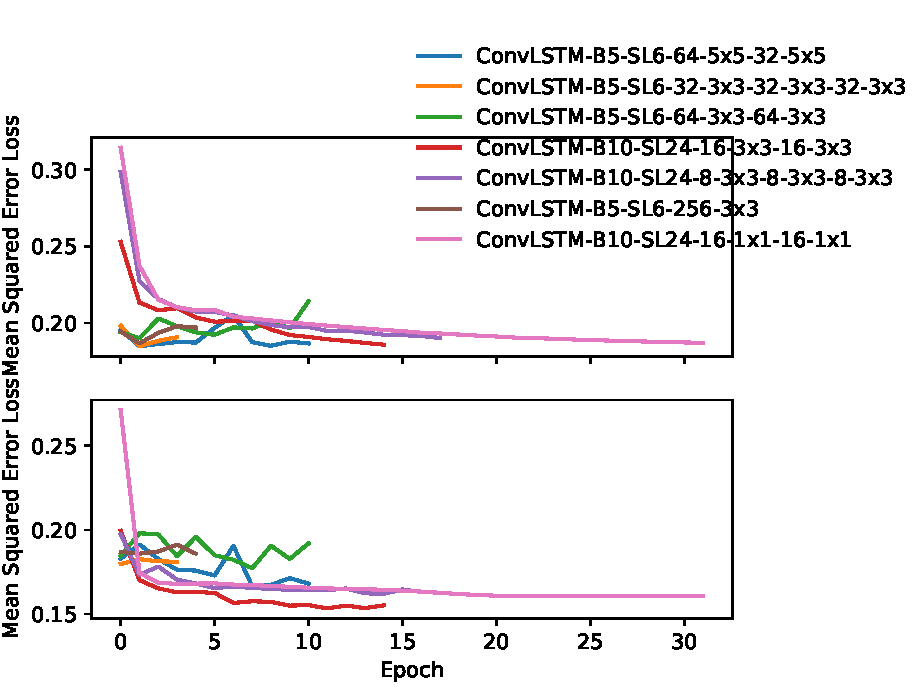
\includegraphics{python_figs/test_epoch_loss.pdf}
    \caption{Loss vs epochs for the trained models in this thesis. Subplot train and valid loss. The resulting legend is then only the model names.}
    \label{fig:convlstm_loss}
\end{figure}

\begin{figure}
    \centering
    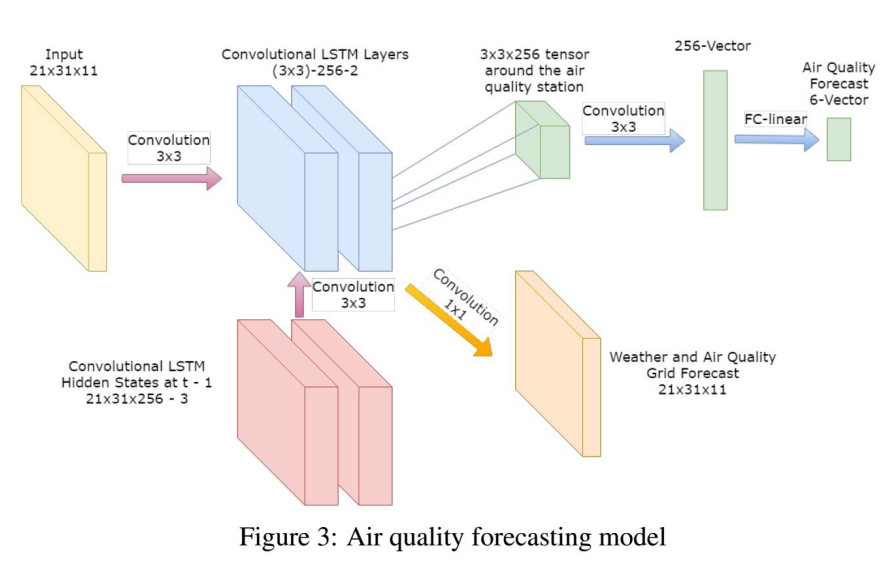
\includegraphics[scale=0.4]{python_figs/example_model.png}
    \caption{Example of how I intend to visualise the best architecture generated for this study.}
    \label{fig:best_ml_architecture}
\end{figure}

\begin{enumerate}
    \item \textbf{TODO: check if it predicts out of sample values if not try and delete samples if it does delete the samples and retrain best model. MAKE table showing max min predicted value over the entire dataset and maybee how many values in percent is out of sample}
\end{enumerate}


 
\subsection{Results on Predicting sequence}
The foundation of the choice of the best model is different for \acrshort{ar} and \acrshort{convlstm}-models. As mentioned in Chapter \ref{ch:num_methods}, the \acrshort{ar}-model is optimized to fit the next timestep, while the \acrshort{convlstm} is optimised to fit a sequence or a prescribed length. In this section the best \acrshort{ar}-model and \acrshort{convlstm}-model are assessed on how well they predict the sequence length of the best \acrshort{convlstm}-model. By feeding the prediction into the \acrshort{ar}-model, one can modify its ability to predict sequences. The two best models are X and Y, with performance measured by the MAE metric of A and B respectively. 

%\subsubsection{Visual Comparison predicting a sequence of length}
Visualizing the experiments for sequences.
%%%% TARGET PREDICITON ERA5
\begin{figure}[ht]
    \centering
    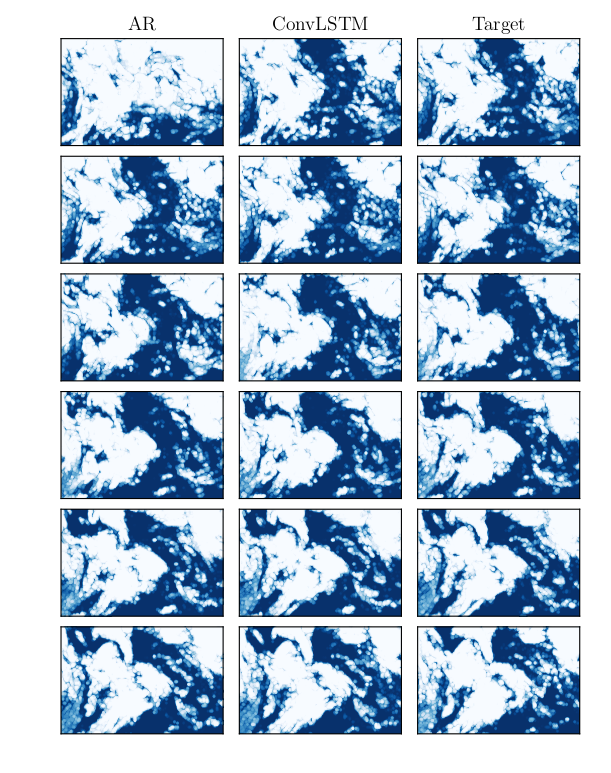
\includegraphics[sale=0.1]{python_figs/example_predicted_sequence_2010-09-01.png}
    \caption{Update figure with real data. Don't think i want to add labels or colorbars the pattern is the most import. \textbf{Trude må jeg ha x og y labels?} }
    \label{fig:target_predict_era5_horizontal}
\end{figure}

Some text where you comment the results from this comparison. Is it evident that the \acrshort{convlstm} is better at predicting spatial patterns as expected or does it all resemble random noise. Is the predicted values in sample or out of sample.


\subsection{Summary} \label{sec:summary_num}
Add text ... 

\clearpage
\section{Practical implications - OUTDATED} \label{sec:practical_implications}
It is necessary to have a understanding of the needs of the end product before conducting large machine learning projects. Answering questions like: What will it be used for and how can it be implemented in useful way?

A major downside of the data driven learning approach is the rigid resolution. A trained model can only be used on similar problems, with the same spatiotemporal resolution. For applications like climate models, output comes in a wide range of different resolutions. Before implementing the finished product in a new model of a different resolution, it would need to be retrained on the resolution of the climate model under development. This process involves both remapping of the dataset and retraining the model at the correct resolution. This is a time consuming process involving finding a new set of hyperparameters suitable for the new resolution. % It essentially means starting over.

Once trained on global climate datasets, machine learning models provide fast results even for complex parameterization which is what makes them suitable for the application of climate modelling. Most machine learning packages are developed using Python. \acrfull{esm} are implemented in python. Methods for including the trained parameterizations need to be developed.
 
\subsection{Any implications based on the results presented in this chapter.}